% +------------------------------------------------------------------------+
% | Reference manual page: TriangulationDataStructure_3.tex
% +------------------------------------------------------------------------+
% | 27.3.2000   Monique Teillaud
% | Package: Triangulation3
% | 
\RCSdef{\RCSTdsRev}{$Revision$}
\RCSdefDate{\RCSTdsDate}{$Date$}
% |
%%RefPage: end of header, begin of main body
% +------------------------------------------------------------------------+


\begin{ccRefConcept}{TriangulationDataStructure_3}

%% \ccHtmlCrossLink{}     %% add further rules for cross referencing links
%% \ccHtmlIndexC[concept]{} %% add further index entries

\ccDefinition

3D-triangulation data structures are meant to maintain the
combinatorial information for 3D-geometric triangulations.

In \cgal, a triangulation data structure is a
container of cells ($3$-faces) and vertices ($0$-faces). Each cell gives
access to its four incident vertices and to its four adjacent
cells. Each vertex gives direct access to one of its incident cells, which is 
sufficient to retrieve all the incident cells when needed.

The four vertices of a cell are indexed with 0, 1, 2 and 3.  The
neighbors of a cell are also indexed with 0, 1, 2, 3 
in such a way that the neighbor indexed by $i$ is opposite to the vertex
with the same index (see Figure~\ref{TDS3-fig-repres}).

Edges ($1$-faces) and facets ($2$-faces) are not explicitly
represented: a facet is given by a cell and an index (the facet
\ccc{i} of a cell \ccc{c} is the facet of \ccc{c} that is opposite to
the vertex of index \ccc{i}) and an edge is given by a cell and two
indices (the edge \ccc{(i,j)} of a cell \ccc{c} is the edge
whose endpoints are the vertices of indices \ccc{i} and \ccc{j} of
\ccc{c}). 

As \cgal\ explicitly deals with all degenerate cases, a
3D-triangulation data structure in \cgal\ can handle the cases when
the dimension of the triangulation is lower than~3 
(see Section~\ref{TDS3-sec-intro}).

Thus, a 3D-triangulation data structure can store a triangulation of a
topological sphere $S^d$ of $\R^{d+1}$, for any $d \in \{-1,0,1,2,3\}$. 

\bigskip

The second template parameter of the basic triangulation class
(see Chapter~\ref{chapter-Triangulation3},
\lcTex{\ccRefPage{CGAL::Triangulation_3<TriangulationTraits_3,TriangulationDataStructure_3>}})
\ccc{Triangulation_3} is a triangulation data structure class. (See
Chapter~\ref{chapter-TDS3}.)  

To ensure all the \textbf{flexibility} of the class \ccc{Triangulation_3}, a
model of a triangulation data structure must be templated by the base vertex
and the base cell classes (see~\ref{TDS3-sec-intro}):
\ccc{TriangulationDataStructure_3<TriangulationVertexBase_3,TriangulationCellBase_3>}.
The optional functionalities related to geometry are compulsory for
this use as a template parameter of \ccc{Triangulation_3}.

\bigskip

A class that satisfies the requirements for a triangulation data structure
class must provide the following types and operations. 

\ccTypes
\ccThree{typedef Triple <Cell_handle, int, int>}{Facet; }{}
\ccThreeToTwo

\ccNestedType{Vertex}{Vertex type}
\ccGlue
\ccNestedType{Cell}{Cell type}

\ccNestedType{size_type}{Size type (unsigned integral type)}
\ccGlue
\ccNestedType{difference_type}{Difference type (signed integral type)}

Vertices and cells are usually manipulated via \ccc{handles}, which support
the two dereference operators \ccc{operator*} and \ccc{operator->}.

\ccNestedType{Vertex_handle}{}
\ccGlue
\ccNestedType{Cell_handle}{}

Requirements for \ccc{Vertex} and \ccc{Cell} are described in
\ccc{TriangulationDataStructure_3::Vertex} and
\ccc{TriangulationDataStructure_3::Cell} \lcTex{(
\ccRefPage{TriangulationDataStructure_3::Vertex} and
\ccRefPage{TriangulationDataStructure_3::Cell})}.

\ccTypedef{typedef Triple<Cell_handle, int, int> Edge;}{\ccc{(c,i,j)} is the
edge of cell \ccc{c} whose vertices indices are \ccc{i} and
\ccc{j}. (See Section~\ref{TDS3-sec-intro}.)}
\ccGlue
\ccTypedef{typedef std::pair<Cell_handle, int>  Facet;}{\ccc{(c,i)} is the facet
of \ccc{c} opposite to the vertex of index \ccc{i}. (See
Section~\ref{TDS3-sec-intro}.)} 

The following iterators allow one to visit all the vertices, edges, facets
and cells of the triangulation data structure. They are all
bidirectional, non-mutable iterators.

\ccNestedType{Cell_iterator}{}
\ccGlue
\ccNestedType{Facet_iterator}{}
\ccGlue
\ccNestedType{Edge_iterator}{}
\ccGlue
\ccNestedType{Vertex_iterator}{}

The following circulators allow us to visit all the cells and facets
incident to a given edge. They are bidirectional and non-mutable.

\ccNestedType{Facet_circulator}{}
\ccGlue
\ccNestedType{Cell_circulator}{}

Iterators and circulators are convertible to the corresponding handles, thus
the user can pass them directly as arguments to the functions.

\ccCreation
\ccCreationVariable{tds}  %% choose variable name
\ccThree{TriangulationDataStructxure_3;}{tds.set_number}{}
\ccThreeToTwo

\ccConstructor{TriangulationDataStructure_3();}
{Default constructor.}

\ccConstructor{TriangulationDataStructure_3(const TriangulationDataStructure_3 & tds1);}
{Copy constructor. All vertices and cells are duplicated.}

\ccMethod{TriangulationDataStructure_3& operator= (const TriangulationDataStructure_3 & tds1);}
{Assignment operator. All vertices and cells are duplicated, and the former
data structure of \ccc{tds} is deleted.}

\ccThree{Vertex_handle_}{tds.insert_in_facet}{}

\ccMethod{Vertex_handle
copy_tds(const TriangulationDataStructure_3 & tds1,
         Vertex_handle v = Vertex_handle());}
{\ccc{tds1} is copied into \ccVar. If $v\, !\!= Vertex_handle()$,
the vertex of \ccVar\ corresponding to \ccc{v} is returned,
otherwise \ccc{Vertex_handle()} is returned.
\ccPrecond{The optional argument \ccc{v} is a vertex of \ccc{tds1}.}}

\ccMethod{void swap(TriangulationDataStructure_3 & tds1);} 
{Swaps \ccVar\ and \ccc{tds1}. There is no copy of cells and vertices,
thus this method runs in constant time. This method should be preferred to
\ccVar=\ccc{tds1} or \ccVar(\ccc{tds1}) when \ccc{tds1} is deleted after
that.}
\ccGlue
\ccMethod{void clear();}
{Deletes all cells and vertices. \ccVar\ is reset as a triangulation
data structure constructed by the default constructor.}

\ccOperations

\ccAccessFunctions
\ccThree{size_type}{tds.insert_in_facet()xxxxxxxxxxx}{}

\ccMethod{int dimension() const;}
{The dimension of the triangulated topological sphere.}
\ccGlue
\ccMethod{size_type number_of_vertices() const;}
{The number of vertices. Note that the triangulation data structure has one
more vertex than an associated geometric triangulation, if there is
one, since the infinite vertex is a standard vertex and is thus also
counted.} 
\ccGlue
\ccMethod{size_type number_of_cells() const;}
{The number of cells. Returns 0 if \ccVar.\ccc{dimension()}$<3$.}

\ccHeading{Non constant-time access functions}
\ccMethod{size_type number_of_facets() const;}
{The number of facets. Returns 0 if \ccVar.\ccc{dimension()}$<2$.}
\ccGlue
\ccMethod{size_type number_of_edges() const;}
{The number of edges. Returns 0 if \ccVar.\ccc{dimension()}$<1$.}

\begin{ccAdvanced}
\ccHeading{Setting}
\ccMethod{void set_dimension(int n);}
{Sets the dimension to \ccc{n}.}
\end{ccAdvanced}

\ccHeading{Queries}

\ccMethod{bool is_vertex(Vertex_handle v) const;}
{Tests whether \ccc{v} is a vertex of \ccVar.}

\ccMethod{bool is_edge(Cell_handle c, int i, int j) const;}
{Tests whether \ccc{(c,i,j)} is an edge of \ccVar. Answers \ccc{false} when
\ccc{dimension()} $<1$ .
\ccPrecond{$i,j \in \{0,1,2,3\}$}}
\ccGlue
\ccMethod{bool is_edge(Vertex_handle u, Vertex_handle v, 
			Cell_handle & c, int & i, int & j) const;}
{Tests whether \ccc{(u,v)} is an edge of \ccVar. If the edge is found,
it computes a cell \ccc{c} having this edge and the indices \ccc{i}
and \ccc{j} of the vertices \ccc{u} and \ccc{v}, in this order.}
\ccGlue
\ccMethod{bool is_edge(Vertex_handle u, Vertex_handle v) const;}
{Tests whether \ccc{(u,v)} is an edge of \ccVar.}

\ccMethod{ bool is_facet(Cell_handle c, int i) const;}
{Tests whether \ccc{(c,i)} is a facet of \ccVar. Answers \ccc{false} when
\ccc{dimension()} $<2$ .
\ccPrecond{$i \in \{0,1,2,3\}$}}
\ccGlue
\ccMethod{bool is_facet(Vertex_handle u, Vertex_handle v, Vertex_handle w, 
			Cell_handle & c, int & i, int & j, int & k) const;}
{Tests whether \ccc{(u,v,w)} is a facet of \ccVar. If the facet is found,
it computes a cell \ccc{c} having this facet and the indices \ccc{i},
\ccc{j} and \ccc{k} of the vertices \ccc{u}, \ccc{v} and \ccc{w}, in
this order.} 

\ccMethod{bool is_cell(Cell_handle c) const;}
{Tests whether \ccc{c} is a cell of \ccVar. Answers \ccc{false} when
\ccc{dimension()} $<3$ .}
\ccMethod{bool is_cell(Vertex_handle u, Vertex_handle v, Vertex_handle w, Vertex_handle t,
			Cell_handle & c, int & i, int & j, int & k, int & l) const;}
{Tests whether \ccc{(u,v,w,t)} is a cell of \ccVar. If the cell
\ccc{c} is found, it computes the indices \ccc{i}, \ccc{j}, \ccc{k}
and \ccc{l} of the vertices \ccc{u}, \ccc{v}, \ccc{w} and \ccc{t} in
\ccc{c}, in this order.} 

There is a method \ccc{has_vertex} in the cell class. The analogous
methods for facets are defined here.

\ccMethod{bool has_vertex(const Facet & f, Vertex_handle v, int & j) const;}
{If \ccc{v} is a vertex of \ccc{f}, then \ccc{j} is the index of
\ccc{v} in the cell \ccc{f.first}, and the method returns \ccc{true}.
\ccPrecond{\ccVar.dimension()=3}}
\ccGlue
\ccMethod{bool has_vertex(Cell_handle c, int i, Vertex_handle v, int & j) const;}
{Same for facet \ccc{(c,i)}. Computes the index \ccc{j} of \ccc{v} in
\ccc{c}.}
\ccGlue
\ccMethod{bool has_vertex(const Facet & f, Vertex_handle v) const;}
{}
\ccGlue
\ccMethod{bool has_vertex(Cell_handle c, int i, Vertex_handle v) const;}
{Same as the first two methods, but these two methods do not return the
index of the vertex.}

The following three methods test whether two facets have the same
vertices.

\ccMethod{bool are_equal(const Facet & f, const Facet & g) const;}
{}
\ccGlue
\ccMethod{bool are_equal(Cell_handle c, int i, Cell_handle n, int j) const;}
{}
\ccGlue
\ccMethod{bool are_equal(const Facet & f, Cell_handle n, int j) const;}
{For these three methods: \ccPrecond{\ccVar.dimension()=3}.}

\ccHeading{Flips}

Two kinds of flips exist for a three-dimensional triangulation. They
are reciprocal. To be flipped, an edge must be incident to three
tetrahedra. During the flip, these three tetrahedra disappear and two
tetrahedra appear. Figure~\ref{TDS3-fig-flips}(left) shows the
edge that is flipped as bold dashed, and one of its three incident
facets is shaded. On the right, the facet shared by the two new
tetrahedra is shaded. 

%Flips are possible only if the tetrahedra to be created do not already 
%exist.

\begin{figure}
\begin{ccTexOnly}
\begin{center} 
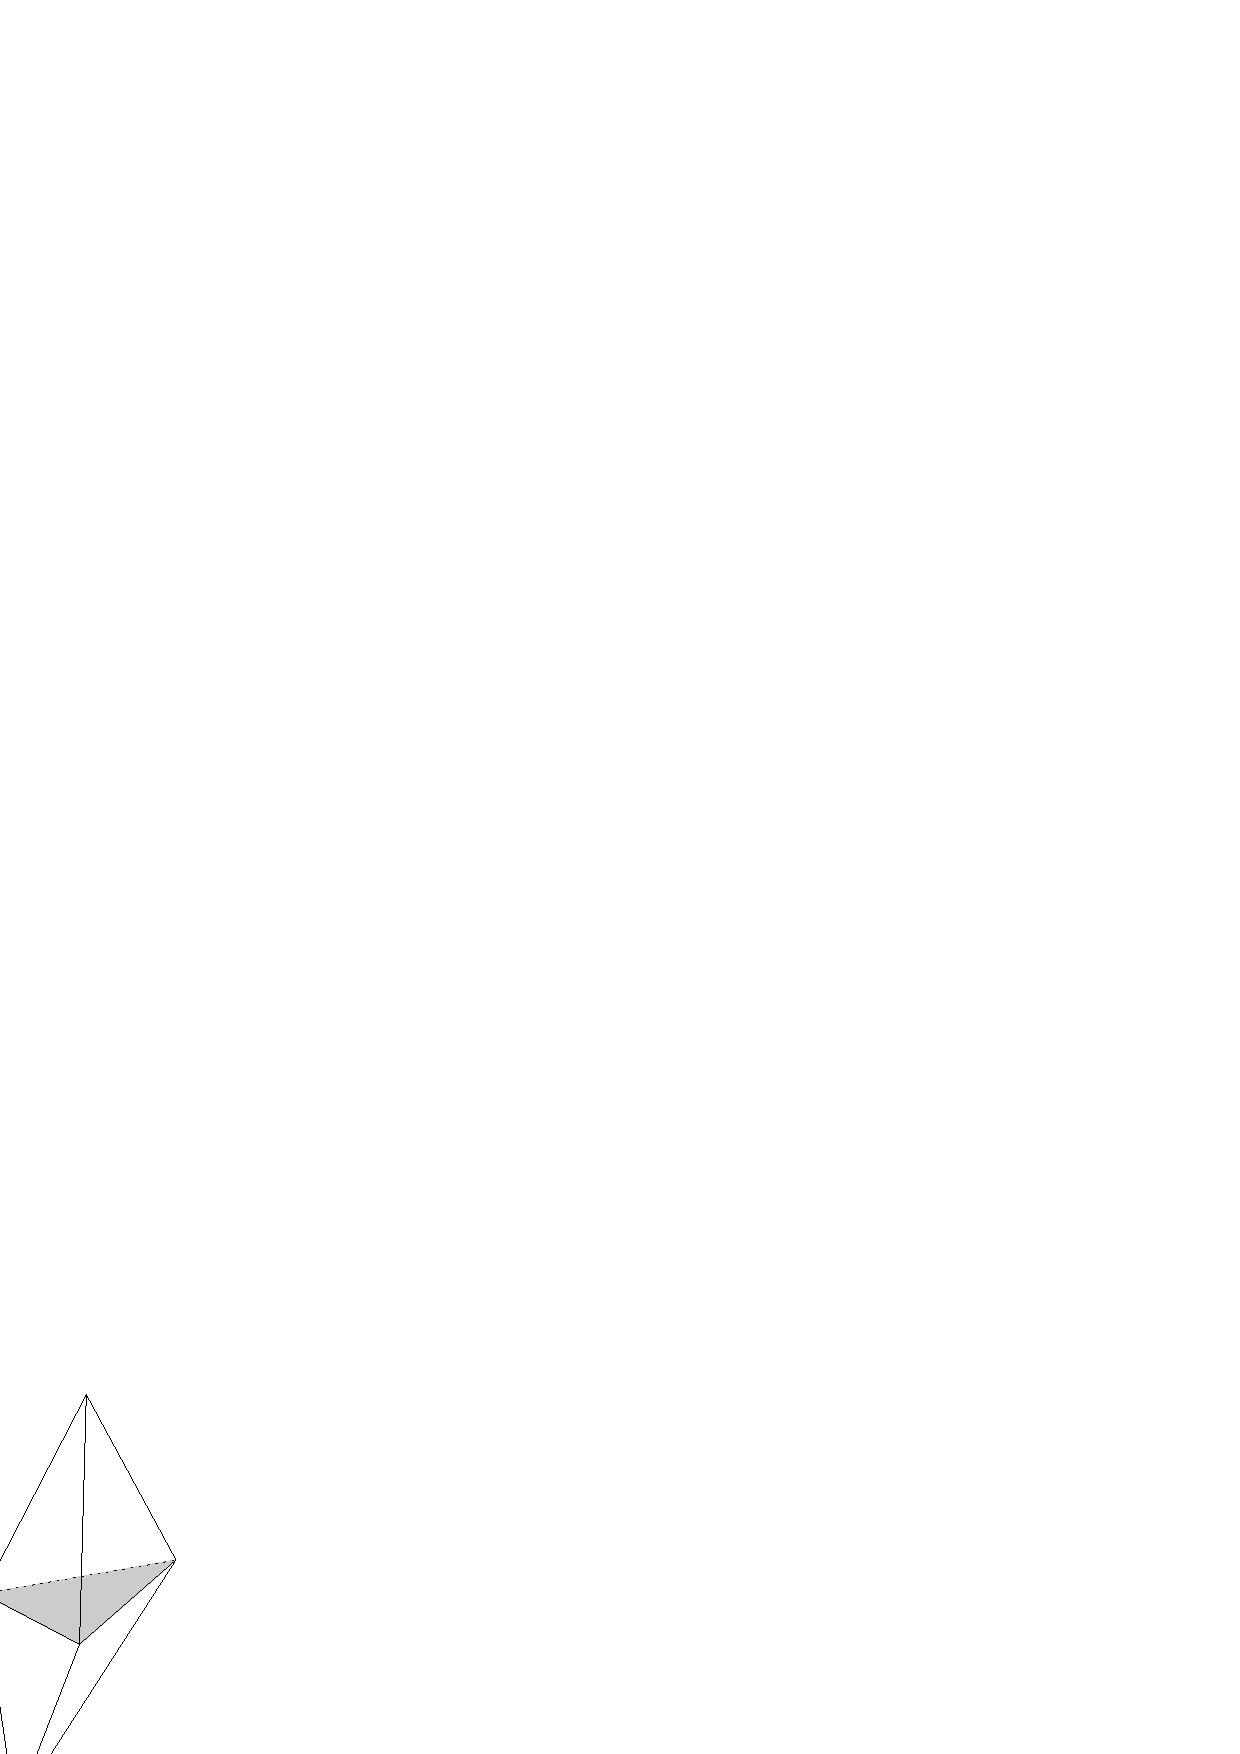
\includegraphics{TriangulationDS_3/flips}
\end{center}
\end{ccTexOnly}
\caption{Flips.
\label{TDS3-fig-flips}}
\begin{ccHtmlOnly}
<CENTER>
<img border=0 src="./flips.gif" align=center
alt="Flips">
</CENTER>
\end{ccHtmlOnly}
\end{figure} 

The following methods guarantee the validity of the resulting 3D
combinatorial triangulation.  Moreover the flip operations do not
invalidate the vertex handles, and only invalidate the cell
handles of the affected cells.

\textit{Flips for a 2d triangulation are not implemented yet}

\ccMethod{bool flip(Edge e);}{}
\ccGlue
\ccMethod{bool flip(Cell_handle c, int i, int j);}
{Before flipping, these methods check that edge \ccc{e=(c,i,j)} is
flippable (which is quite expensive). They return \ccc{false} or
\ccc{true} according to this test.}

\ccMethod{void flip_flippable(Edge e);}{}
\ccGlue
\ccMethod{void flip_flippable(Cell_handle c, int i, int j);}
{Should be preferred to the previous methods when the edge is
known to be flippable.
\ccPrecond{The edge is flippable.}}

\ccMethod{bool flip(Facet f);}{}
\ccGlue
\ccMethod{bool flip(Cell_handle c, int i);}
{Before flipping, these methods check that facet \ccc{f=(c,i)} is
flippable (which is quite expensive). They return \ccc{false} or
\ccc{true} according to this test.} 

\ccMethod{void flip_flippable(Facet f);}{}
\ccGlue
\ccMethod{void flip_flippable(Cell_handle c, int i);}
{Should be preferred to the previous methods when the facet is
known to be flippable.
\ccPrecond{The facet is flippable.}}

\ccHeading{Insertions}
\ccThree{Vertex_handle}{tds.insert_in_facet()xxxxx}{}

The following modifier member functions guarantee
the combinatorial validity of the resulting triangulation.

\ccMethod{Vertex_handle insert_in_cell(Cell_handle c);} 
{Creates a new vertex, inserts it in cell \ccc{c} and returns its handle.
The cell \ccc{c} is split into four new cells, each of these cells being
formed by the new vertex and a facet of \ccc{c}.
\ccPrecond{\ccVar.\ccc{dimension()} $= 3$ and \ccc{c} is a cell of \ccVar.}}

\ccMethod{Vertex_handle insert_in_facet(const Facet & f);} 
{Creates a new vertex, inserts it in facet \ccc{f} and returns its handle.
In dimension 3, the two incident cells are split into 3 new cells;
in dimension 2, the facet is split into 3 facets.
\ccPrecond{\ccVar.\ccc{dimension()} $\geq 2$ and \ccc{f} is a
facet of \ccVar.}} 

\ccMethod{Vertex_handle insert_in_facet(Cell_handle c, int i);} 
{Creates a new vertex, inserts it in facet \ccc{i} of \ccc{c} and returns its
handle.
\ccPrecond{\ccVar.\ccc{dimension()} $\geq 2$, $i \in \{0,1,2,3\}$ 
in dimension~3, $i=3$ in dimension~2 and \ccc{(c,i)} is a facet of
\ccVar.}} 

\ccMethod{Vertex_handle insert_in_edge(Edge e);} 
{Creates a new vertex, inserts it in edge \ccc{e} and returns its handle.
In dimension 3, all the
incident cells are split into 2 new cells; in dimension 2, the 2
incident facets are split into 2 new facets; in dimension 1, the edge is 
split into 2 new edges.
\ccPrecond{\ccVar.\ccc{dimension()} $\geq 1$ and \ccc{e} is an edge of
\ccVar.}} 

\ccMethod{Vertex_handle insert_in_edge(Cell_handle c, int i, int j);} 
{Creates a new vertex, inserts it in edge $(i,j)$ of \ccc{c} and returns its
handle.
\ccPrecond{\ccVar.\ccc{dimension()} $\geq 1$. $i\neq j$, $i,j \in
\{0,1,2,3\}$ in dimension~3, $i,j \in \{0,1,2\}$ in dimension~2, $i,j
\in \{0,1\}$ in dimension~1 and \ccc{(c,i,j)} is an edge of \ccVar.}}

\ccMethod{Vertex_handle
          insert_increase_dimension(Vertex_handle star = Vertex_handle());}
{Transforms a triangulation of the sphere $S^d$ of $\R^{d+1}$ into the
triangulation of the sphere $S^{d+1}$ of $\R^{d+2}$ by adding a new vertex
\ccc{v}:  
\ccc{v} is linked to all the vertices to triangulate one of the two
halfspheres of dimension $(d+1)$. Vertex \ccc{star} is used to
triangulate the second halfsphere (when there is an associated
geometric triangulation, \ccc{star} is in fact the vertex associated with
its infinite vertex).
See Figure~\ref{TDS3-fig-topo-insert_outside_affine_hull}.\\  
The numbering of the cells is such that, if \ccc{f} was a face of
maximal dimension in the initial triangulation, then \ccc{(f,v)} (in
this order) is the corresponding face in the new triangulation.
This method can be used to insert the first two vertices in an empty
triangulation.\\
A handle to \ccc{v} is returned.
\ccPrecond{\ccVar.\ccc{dimension()} $= d < 3$. When
\ccVar.\ccc{number_of_vertices()} $>0$, $star \neq Vertex_handle()$ and
\ccc{star} is a vertex of \ccVar.}} 

\begin{figure}[htbp]
\begin{ccTexOnly}
\begin{center} 
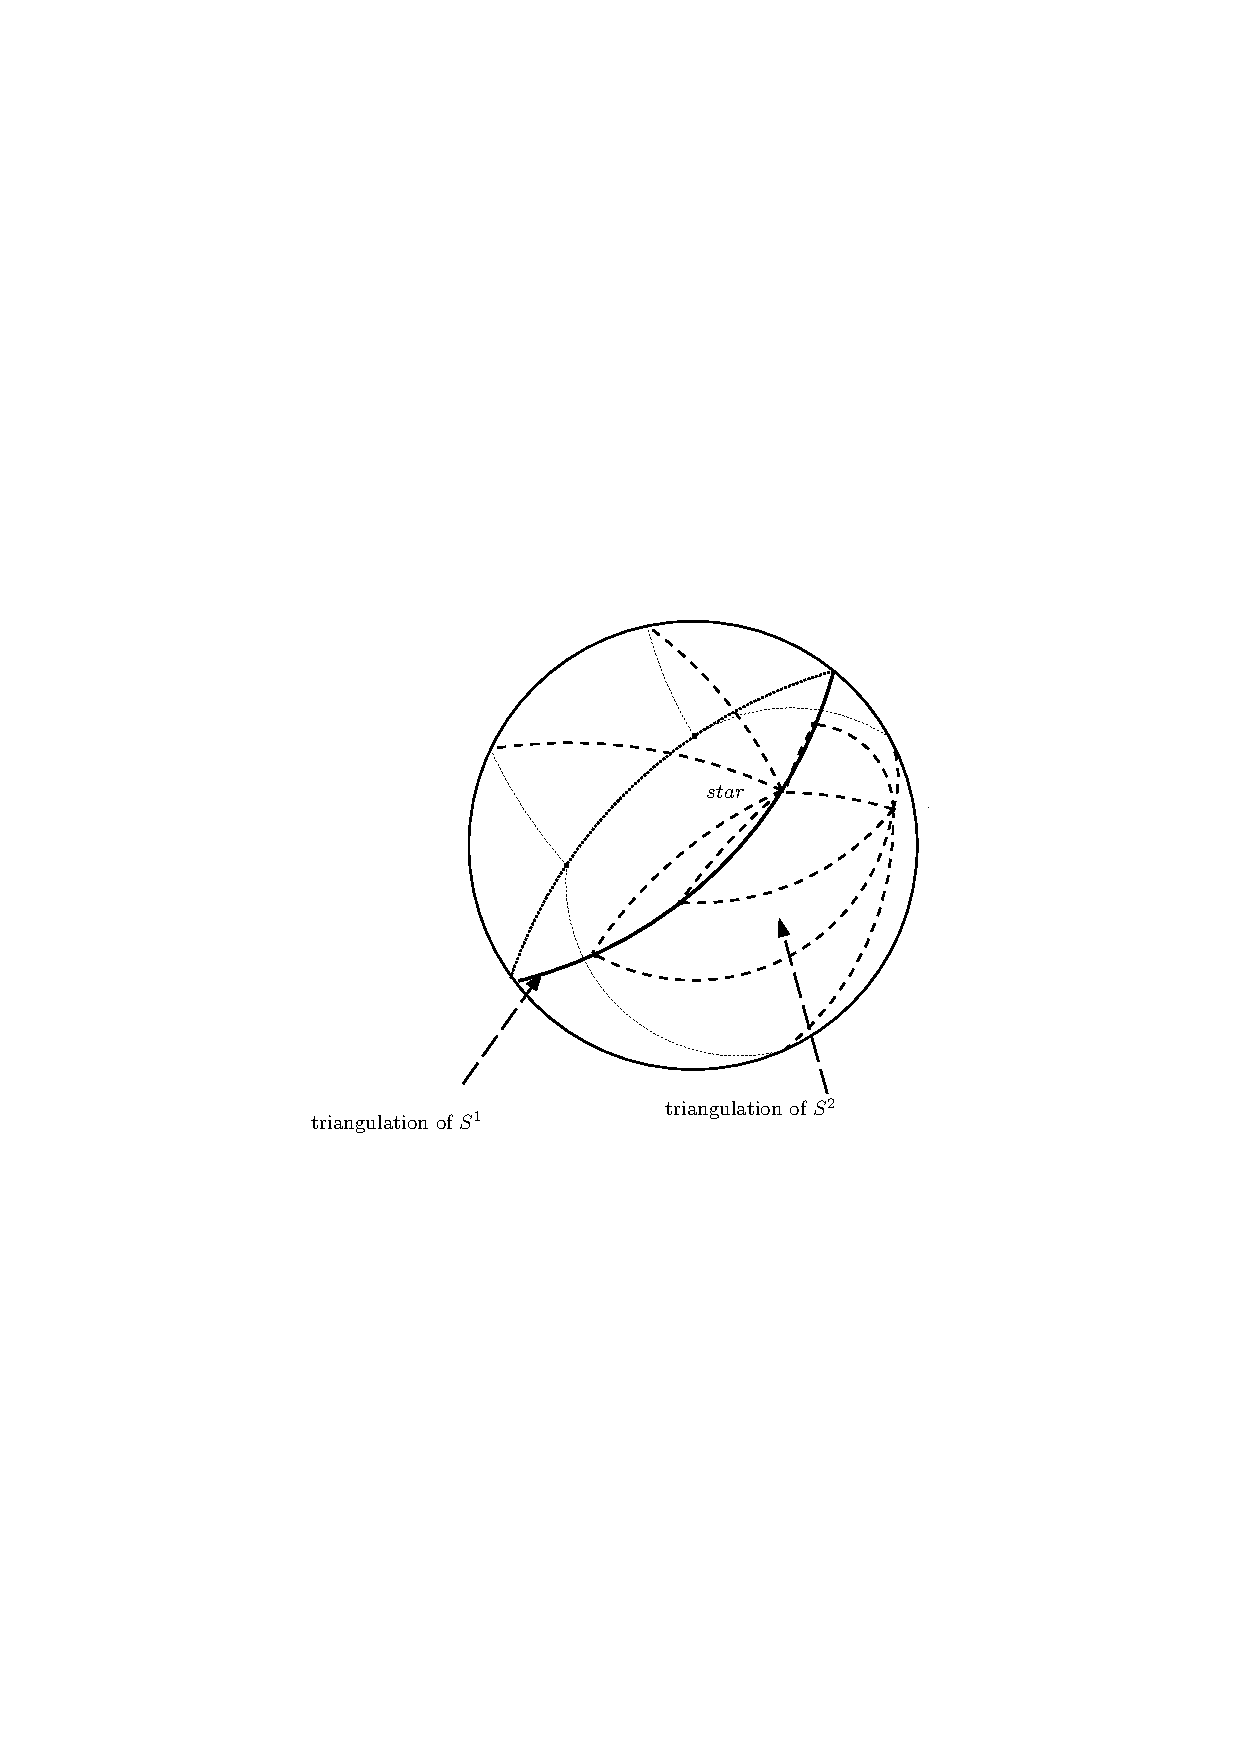
\includegraphics{TriangulationDS_3_ref/topo-insert_outside_affine_hull} 
\end{center}
\end{ccTexOnly}
\caption{\protect\ccc{insert_increase_dimension} (1-dimensional case).
\label{TDS3-fig-topo-insert_outside_affine_hull}}
\begin{ccHtmlOnly}
<CENTER>
<img border=0 src="./topo-insert_outside_affine_hull.gif" align=center
alt="insert_increase_dimension} (1-dimensional case)">
</CENTER>
\end{ccHtmlOnly}
\end{figure} 

\ccMethod{template <class CellIt>
          Vertex_handle insert_in_hole(CellIt cell_begin, CellIt cell_end,
	                               Cell_handle begin, int i);}
{Creates a new vertex by starring a hole.  It takes an iterator range
[\ccc{cell_begin}; \ccc{cell_end}[ of \ccc{Cell_handles} which specifies a set
of connected cells (resp. facets in dimension 2) describing a hole.
(\ccc{begin}, \ccc{i}) is a facet (resp. an edge) on the boundary of the hole,
that is, \ccc{begin} belongs to the set of cells (resp.  facets) previously
described, and \ccc{begin->neighbor(i)} does not.  Then this function deletes
all the cells (resp. facets) describing the hole, creates a new vertex
\ccc{v}, and for each facet (resp. edge) on the boundary of the hole, creates
a new cell (resp. facet) with \ccc{v} as vertex.  \ccc{v} is returned.
\ccPrecond{\ccVar.\ccc{dimension()} $\geq 2$, the set of cells (resp. facets)
is connected, and its boundary is connected.}}

\ccHeading{Removal}

\ccMethod{void remove_decrease_dimension(Vertex_handle v, Vertex_handle w = v);}
{This operation is the reciprocal of \ccc{insert_increase_dimension()}.
It transforms a triangulation of the sphere $S^d$ of $\R^{d+1}$ into the
triangulation of the sphere $S^{d-1}$ of $\R^{d}$ by removing the vertex
\ccc{v}. Delete the cells incident to \ccc{w}, keep the others.
\ccPrecond{\ccVar.\ccc{dimension()} $= d \geq -1$.
\ccVar.\ccc{degree(v)} $=$ \ccc{degree(w)} $=$ \ccVar.\ccc{number_of_vertices()} $-1$.}
}

\ccMethod{Cell_handle remove_from_maximal_dimension_simplex(Vertex_handle v);}
{Removes \ccc{v}. The incident simplices of maximal dimension incident to
\ccc{v} are replaced by a single simplex of the same dimension. This
operation is exactly the reciprocal to \ccVar.\ccc{insert_in_cell(v)} in
dimension 3, \ccVar.\ccc{insert_in_facet(v)} in dimension 2, and
\ccVar.\ccc{insert_in_edge(v)} in dimension 1.
\ccPrecond{\ccVar.\ccc{degree(v)} $=$ \ccVar.\ccc{dimension()+1}.}
}


\begin{ccAdvanced}
\ccHeading{Other modifiers}
The following modifiers can affect the validity of the triangulation
data structure.

\ccMethod{void reorient();}
{Changes the orientation of all cells of the triangulation data structure.
\ccPrecond{\ccVar.\ccc{dimension()} $\geq 1$.}}

\ccMethod{Vertex_handle create_vertex(const Vertex &v = Vertex());}
{Adds a copy of the vertex \ccc{v} to the triangulation data structure.}

\ccMethod{Vertex_handle create_vertex(Vertex_handle v);}
{Creates a vertex which is a copy of the one pointed to by \ccc{v}
and adds it to the triangulation data structure.}

\ccMethod{Cell_handle create_cell(const Cell &c = Cell());}
{Adds a copy of the cell \ccc{c} to the triangulation data structure.}

\ccMethod{Cell_handle create_cell(Cell_handle c);}
{Creates a cell which is a copy of the one pointed to by \ccc{c}
and adds it to the triangulation data structure.}

\ccMethod{Cell_handle create_cell(Vertex_handle v0, Vertex_handle v1,
                                  Vertex_handle v2, Vertex_handle v3);}
{Creates a cell and adds it into the triangulation data
structure. Initializes the vertices of the cell, its neighbor handles
being initialized with the default constructed handle.}

\ccMethod{Cell_handle create_cell( Vertex_handle v0, Vertex_handle v1,
                                   Vertex_handle v2, Vertex_handle v3,
		                   Cell_handle n0, Cell_handle n1,
                                   Cell_handle n2, Cell_handle n3);}
{Creates a cell, initializes its vertices and neighbors, and adds it
into the triangulation data structure.}

\ccMethod{void delete_vertex( Vertex_handle v );}
{Removes the vertex from the triangulation data structure.
\ccPrecond{The vertex is a vertex of \ccVar.}}

\ccMethod{void delete_cell( Cell_handle c );}
{Removes the cell from the triangulation data structure.
\ccPrecond{The cell is a cell of \ccVar.}}

\ccMethod{template <class VertexIt>
          void delete_vertices(VertexIt first, VertexIt last);}
{Calls \ccc{delete_vertex} over an iterator range of value type
\ccc{Vertex_handle}.}

\ccMethod{template <class CellIt>
          void delete_cells(CellIt first, CellIt last);}
{Calls \ccc{delete_cell} over an iterator range of value type
\ccc{Cell_handle}.}

\end{ccAdvanced}

\ccHeading{Traversing the triangulation}
\ccThree{Facet_circulator}{tds.vertices_begin()()}{}

\ccMethod{Cell_iterator cells_begin() const;}
{Returns \ccc{cells_end()} when \ccVar.\ccc{dimension()}~$<3$.}
\ccGlue
\ccMethod{Cell_iterator cells_end() const;}{}
\ccGlue
\ccMethod{Cell_iterator raw_cells_begin() const;}
{Low-level access to the cells, does not return \ccc{cells_end()}
when \ccVar.\ccc{dimension()}~$<3$.}
\ccGlue
\ccMethod{Cell_iterator raw_cells_end() const;}{}
\ccGlue
\ccMethod{Facet_iterator facets_begin() const;}
{Returns \ccc{facets_end()} when \ccVar.\ccc{dimension()}~$<2$.}
\ccGlue
\ccMethod{Facet_iterator facets_end() const;}{}
\ccGlue
\ccMethod{Edge_iterator edges_begin() const;}
{Returns \ccc{edges_end()} when \ccVar.\ccc{dimension()}~$<1$.}
\ccGlue
\ccMethod{Edge_iterator edges_end() const;}{}
\ccGlue
\ccMethod{Vertex_iterator vertices_begin() const;}{}
\ccGlue
\ccMethod{Vertex_iterator vertices_end() const;}{}

\ccThree{Facet_circulator}{tds.inciden__cells}{}

\ccMethod{Cell_circulator incident_cells(const Edge & e) const;}
{Starts at an arbitrary cell incident to \ccc{e}.
\ccPrecond{\ccVar.\ccc{dimension()}~$=3$}}
\ccGlue
\ccMethod{Cell_circulator incident_cells(Cell_handle c, int i, int j) const;}
{As above for edge \ccc{(i,j)} of \ccc{c}.}
\ccGlue
\ccMethod{Cell_circulator incident_cells(const Edge & e, Cell_handle start) const;}
{Starts at cell \ccc{start}.
\ccPrecond{\ccVar.\ccc{dimension()}~$=3$ and \ccc{start} is incident to
\ccc{e}.}}
\ccGlue
\ccMethod{Cell_circulator incident_cells(Cell_handle c, int i, int j, Cell_handle start)
const;}
{As above for edge \ccc{(i,j)} of \ccc{c}.}

The following circulators on facets are defined only in dimension~3,
though facets are defined also in dimension~2: there are only two
facets sharing an edge in dimension~2. 
\ccMethod{Facet_circulator incident_facets(Edge e) const;}
{Starts at an arbitrary facet incident to \ccc{e}.
\ccPrecond{\ccVar.\ccc{dimension()}~$=3$}} 
\ccGlue
\ccMethod{Facet_circulator incident_facets(Cell_handle c, int i, int j) const;}
{As above for edge \ccc{(i,j)} of \ccc{c}.} 
\ccGlue
\ccMethod{Facet_circulator incident_facets(Edge e, Facet start) const;}
{Starts at facet \ccc{start}.
\ccPrecond{\ccc{start} is incident to \ccc{e}.}}
\ccGlue
\ccMethod{Facet_circulator incident_facets(Edge e, Cell_handle start, int f) const;}
{Starts at facet of index \ccc{f} in \ccc{start}.}
\ccGlue
\ccMethod{Facet_circulator incident_facets(Cell_handle c, int i, int j,
Facet start) const;} 
{As above for edge \ccc{(i,j)} of \ccc{c}.} 
\ccGlue
\ccMethod{Facet_circulator incident_facets(Cell_handle c, int i, int j,
Cell_handle start, int f) const;}
{As above for edge \ccc{(i,j)} of \ccc{c} and facet \ccc{(start,f)}.} 

\ccHeading{Traversal of the incident cells and facets, and the
adjacent vertices of a given vertex}

\ccThree{void_circulator}{tds.facets_begin()toto}{}

\ccMethod{template <class OutputIterator>
          OutputIterator
          incident_cells(Vertex_handle v, OutputIterator cells) const;}
{Copies the \ccc{Cell_handle}s of all cells (resp. facets in dimension 2)
incident to \ccc{v} to the output iterator \ccc{cells}.
If \ccVar.\ccc{dimension()} $<2$, then do nothing.
Returns the resulting output iterator.
\ccPrecond{\ccc{v} $\neq$ \ccc{Vertex_handle()}, \ccVar.\ccc{is_vertex(v)}.}}

\ccMethod{template <class OutputIterator>
          OutputIterator
          incident_facets(Vertex_handle v, OutputIterator facets) const;}
{Copies the \ccc{Facet}s incident to \ccc{v} to the output iterator
\ccc{facets}.
Returns the resulting output iterator.
\ccPrecond{\ccVar.\ccc{dimension()} $=3$, \ccc{v} $\neq$ \ccc{Vertex_handle()}, \ccVar.\ccc{is_vertex(v)}.}}

\ccMethod{template <class OutputIterator>
          OutputIterator
          incident_vertices(Vertex_handle v, OutputIterator vertices) const;}
{Copies the \ccc{Vertex_handle}s of all vertices incident to \ccc{v} to the
output iterator \ccc{vertices}.  If \ccVar.\ccc{dimension()} $<2$, then do
nothing.  Returns the resulting output iterator.
\ccPrecond{\ccc{v} $\neq$ \ccc{Vertex_handle()}, \ccVar.\ccc{is_vertex(v)}.}}

\ccMethod{size_type degree(Vertex_handle v) const;}
{Returns the degree of a vertex, that is, the number of incident vertices.
\ccPrecond{\ccc{v} $\neq$ \ccc{Vertex_handle()}, \ccVar.\ccc{is_vertex(v)}.}}

\ccMethod{int mirror_index(Cell_handle c, int i) const;}
{Returns the index of \ccc{c} in its $i^{th}$ neighbor.
\ccPrecond{$i \in \{0, 1, 2, 3\}$.}}
\ccGlue
\ccMethod{Vertex_handle mirror_vertex(Cell_handle c, int i) const;}
{Returns the vertex of the $i^{th}$ neighbor of \ccc{c} that is opposite to
\ccc{c}.
\ccPrecond{$i \in \{0, 1, 2, 3\}$.}}
\ccGlue
\ccMethod{Facet mirror_facet(Facet f) const;}
{Returns the same facet viewed from the other adjacent cell.}


\begin{ccAdvanced}
\ccHeading{Checking}

\ccMethod{bool is_valid(bool verbose = false) const;}
{Checks the combinatorial validity of the triangulation by checking
the local validity of all its cells and vertices (see functions below). 
(See Section~\ref{TDS3-sec-intro}.) Moreover, the Euler relation is
tested.\\
When \ccc{verbose} is set to \ccc{true}, messages are printed to give
a precise indication on the kind of invalidity encountered.}

\ccMethod{bool is_valid(Vertex_handle v, bool verbose = false) const;}
{Checks the local validity of the adjacency relations of the triangulation.
It also calls the \ccc{is_valid} member function of the vertex.
When \ccc{verbose} is set to \ccc{true}, messages are printed to give
a precise indication on the kind of invalidity encountered.}

\ccMethod{bool is_valid(Cell_handle c, bool verbose = false) const;}
{Checks the local validity of the adjacency relations of the triangulation.
It also calls the \ccc{is_valid} member function of the cell.
When \ccc{verbose} is set to \ccc{true}, messages are printed to give
a precise indication on the kind of invalidity encountered.}

\end{ccAdvanced}

\ccHeading{I/O}

\ccFunction{istream& operator>>
	(istream& is, TriangulationDataStructure_3 & tds);}
{Reads a combinatorial triangulation from \ccc{is} and assigns it to \ccc{tds}}

\ccFunction{ostream& operator<<
	(ostream& os, const TriangulationDataStructure_3 & tds);}
{Writes \ccc{tds} into the stream \ccc{os}}

The information stored in the \ccc{iostream} is: 
the dimension, the number of vertices, the number of cells,
the indices of the vertices of each cell, then the indices of the
neighbors of each cell, where the index corresponds to the preceding
list of cells. When dimension $<$ 3, the same information is stored
for faces of maximal dimension instead of cells.

\ccHasModels

\ccc{CGAL::Triangulation_data_structure_3}

\ccSeeAlso

\ccc{TriangulationDataStructure_3::Vertex}\\
\ccc{TriangulationDataStructure_3::Cell}

\end{ccRefConcept}
